\documentclass[hyperref, a4paper]{article}

\usepackage{geometry}
\usepackage{titling}
\usepackage{titlesec}
% No longer needed, since we will use enumitem package
% \usepackage{paralist}
\usepackage{enumitem}
\usepackage{footnote}
\usepackage{enumerate}
\usepackage{amsmath, amssymb, amsthm}
\usepackage{mathtools}
\usepackage{bbm}
\usepackage{graphicx}
\usepackage{subcaption}
\usepackage{physics}
\usepackage{tensor}
\usepackage{siunitx}
\usepackage[version=4]{mhchem}
\usepackage{tikz}
\usepackage{xcolor}
\usepackage{listings}
\usepackage{autobreak}
\usepackage[ruled, vlined, linesnumbered]{algorithm2e}
\usepackage{nameref,zref-xr}
\zxrsetup{toltxlabel}
\usepackage[sorting=none]{biblatex}
\bibliography{squeezing}
\usepackage[colorlinks,unicode]{hyperref} % , linkcolor=black, anchorcolor=black, citecolor=black, urlcolor=black, filecolor=black
\usepackage[most]{tcolorbox}
\usepackage{prettyref}

% Page style
\geometry{left=3.18cm,right=3.18cm,top=2.54cm,bottom=2.54cm}
\titlespacing{\paragraph}{0pt}{1pt}{10pt}[20pt]
\setlength{\droptitle}{-5em}

% More compact lists 
\setlist[itemize]{
    itemindent=17pt, 
    leftmargin=1pt,
    listparindent=\parindent,
    parsep=0pt,
}

% Math operators
\DeclareMathOperator{\timeorder}{\mathcal{T}}
\DeclareMathOperator{\diag}{diag}
\DeclareMathOperator{\legpoly}{P}
\DeclareMathOperator{\primevalue}{P}
\DeclareMathOperator{\sgn}{sgn}
\DeclareMathOperator{\res}{Res}
\newcommand*{\ii}{\mathrm{i}}
\newcommand*{\ee}{\mathrm{e}}
\newcommand*{\const}{\mathrm{const}}
\newcommand*{\suchthat}{\quad \text{s.t.} \quad}
\newcommand*{\argmin}{\arg\min}
\newcommand*{\argmax}{\arg\max}
\newcommand*{\normalorder}[1]{: #1 :}
\newcommand*{\pair}[1]{\langle #1 \rangle}
\newcommand*{\fd}[1]{\mathcal{D} #1}
\DeclareMathOperator{\bigO}{\mathcal{O}}

% TikZ setting
\usetikzlibrary{arrows,shapes,positioning}
\usetikzlibrary{arrows.meta}
\usetikzlibrary{decorations.markings}
\tikzstyle arrowstyle=[scale=1]
\tikzstyle directed=[postaction={decorate,decoration={markings,
    mark=at position .5 with {\arrow[arrowstyle]{stealth}}}}]
\tikzstyle ray=[directed, thick]
\tikzstyle dot=[anchor=base,fill,circle,inner sep=1pt]

% Algorithm setting
% Julia-style code
\SetKwIF{If}{ElseIf}{Else}{if}{}{elseif}{else}{end}
\SetKwFor{For}{for}{}{end}
\SetKwFor{While}{while}{}{end}
\SetKwProg{Function}{function}{}{end}
\SetArgSty{textnormal}

\newcommand*{\concept}[1]{{\textbf{#1}}}

% Embedded codes
\lstset{basicstyle=\ttfamily,
  showstringspaces=false,
  commentstyle=\color{gray},
  keywordstyle=\color{blue}
}

% Reference formatting
\newrefformat{fig}{Fig.~\ref{#1}}

% Color boxes
\tcbuselibrary{skins, breakable, theorems}
\newtcbtheorem[number within=section]{warning}{Warning}%
  {colback=orange!5,colframe=orange!65,fonttitle=\bfseries, breakable}{warn}
\newtcbtheorem[number within=section]{note}{Note}%
  {colback=green!5,colframe=green!65,fonttitle=\bfseries, breakable}{note}
\newtcbtheorem[number within=section]{info}{Info}%
  {colback=blue!5,colframe=blue!65,fonttitle=\bfseries, breakable}{info}

\newenvironment{shelldisplay}{\begin{lstlisting}}{\end{lstlisting}}

\title{Squeezing of quantum noise}
\author{Jinyuan Wu}

\begin{document}
    
\maketitle

\begin{abstract}
    Systems isolated from external disturbance still have noises 
    arising from the uncertain nature of quantum observables,
    which set a limit to the precision of linear quantum optics interferometers.
    This report visualizes quantum noise using Wigner function,
    analyzes the quantum noise in Mach-Zehnder interferometer 
    in the small phase difference limit,
    and demonstrates the quantum noise can be ``squeezed''
    by changing the dark port input
    in an intuitive way according to the visualization.
\end{abstract}

\section{Introduction}

Noise usually arises from coupling with an unknown environment:
when we keep our eyes only on one of the system,
we need to average over the state of the environment,
which corrects the equation of motion of the system 
with noise and dissipation \cite{zwanzig_nonequilibrium_2001}.
However, systems isolated from the outside world still have noise:
if the wave function of the system is not an eigenstate of the observable in question, 
any experimental setting measuring that observable has noisy results.
This kind of noise is called \concept{quantum noise}.

In systems that can be well described by 
harmonic oscillators,
for each oscillation mode, 
we have two variables $X$ and $P$, and $[X, P] = \ii$
(here and below we use Planck system of units),
and the Hamiltonian is $H \simeq c_1 X^2 + c_2 P^2$ 
plus possible interaction perturbations.
After diagonalization, we get $H \simeq \sum_{\text{modes}} \omega (a^\dagger a + 1/2)$,
which may be further modified by interaction terms.
The zero-point energy $1/2$ arises from the non-commutative nature of $X$ and $P$.
Another way to see the quantum nature of the zero-point energy is to note that at the ground state,
though $\expval{X} = \expval{P} = 0$,
since we have the zero-point energy,
$\expval*{X^2}, \expval*{P^2} \propto \expval*{H} / 2 \neq 0$.
We therefore sometimes say that 
quantum noise comes from the zero point-energy.
Of course, by manipulating the quantum state, 
the variance of \emph{one} degree of freedom 
may be reduced,
at the cost of larger variances on other degrees of freedom.
This is called ``squeezing'' of the quantum noise.

% We may also consult this:
% Quantum noise and quantum measurement
% https://clerkgroup.uchicago.edu/PDFfiles/LesHouchesNotesAC.pdf

This report focuses on quantum noises in linear quantum optics interferometry,
which fits in the picture described above.
\prettyref{sec:overview-rep} discusses quantitative ways to represent and characterize quantum noise.
\prettyref{sec:interferometer} calculates quantum noise 
in Mach-Zehnder interferometer.
\prettyref{sec:dark-port-analysis} demonstrates that
when the input laser beam is strong enough,
the quantum noise in the output can be attributed to the quantum noise in the dark port.
\prettyref{sec:squeezing} shows how to squeeze the quantum noise in the output 
by injecting a squeezed state into the dark port.

\section{Quantum optics states and quasi-probability distribution functions}\label{sec:overview-rep}

\begin{figure}
    \centering
    \begin{subfigure}{0.45\textwidth}
        \centering
        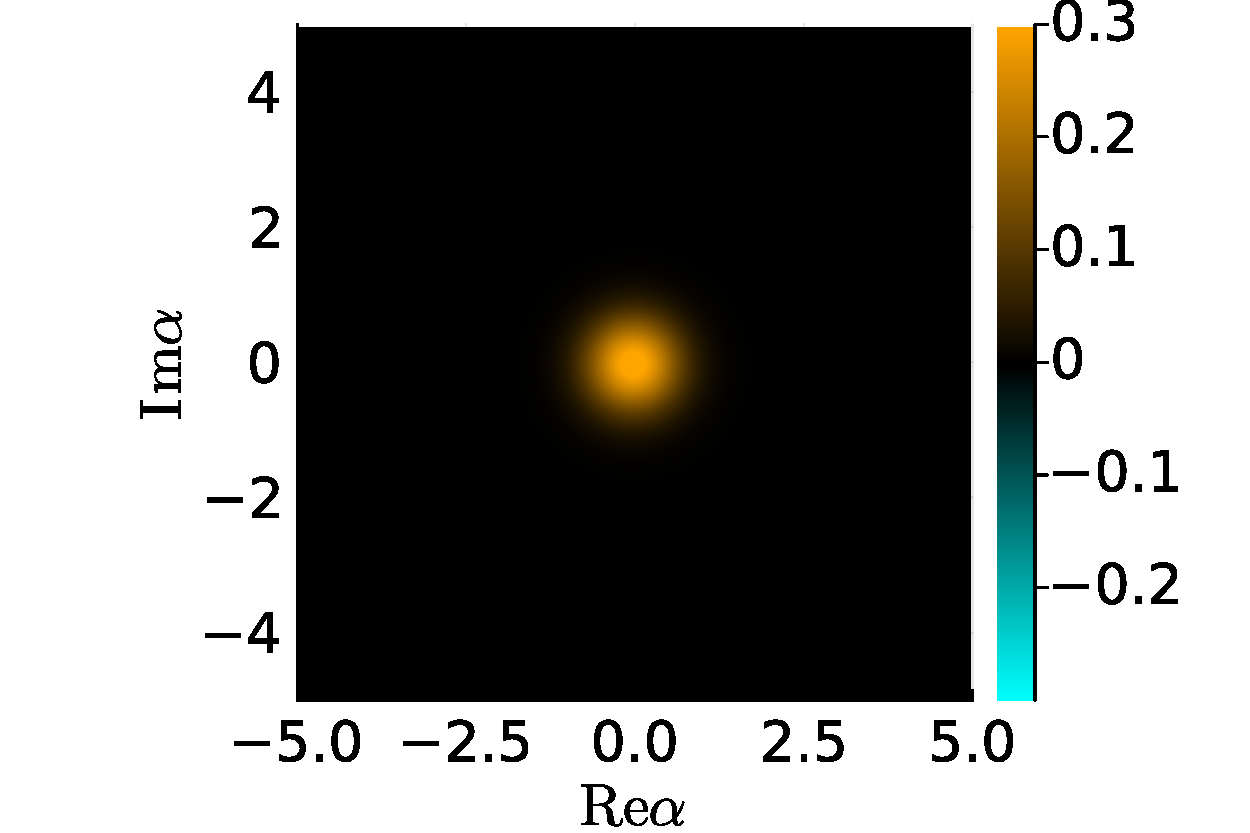
\includegraphics[width=\textwidth]{heatmaps/coherent-state.pdf}
        \subcaption{}
    \end{subfigure}
    \begin{subfigure}{0.45\textwidth}
        \centering
        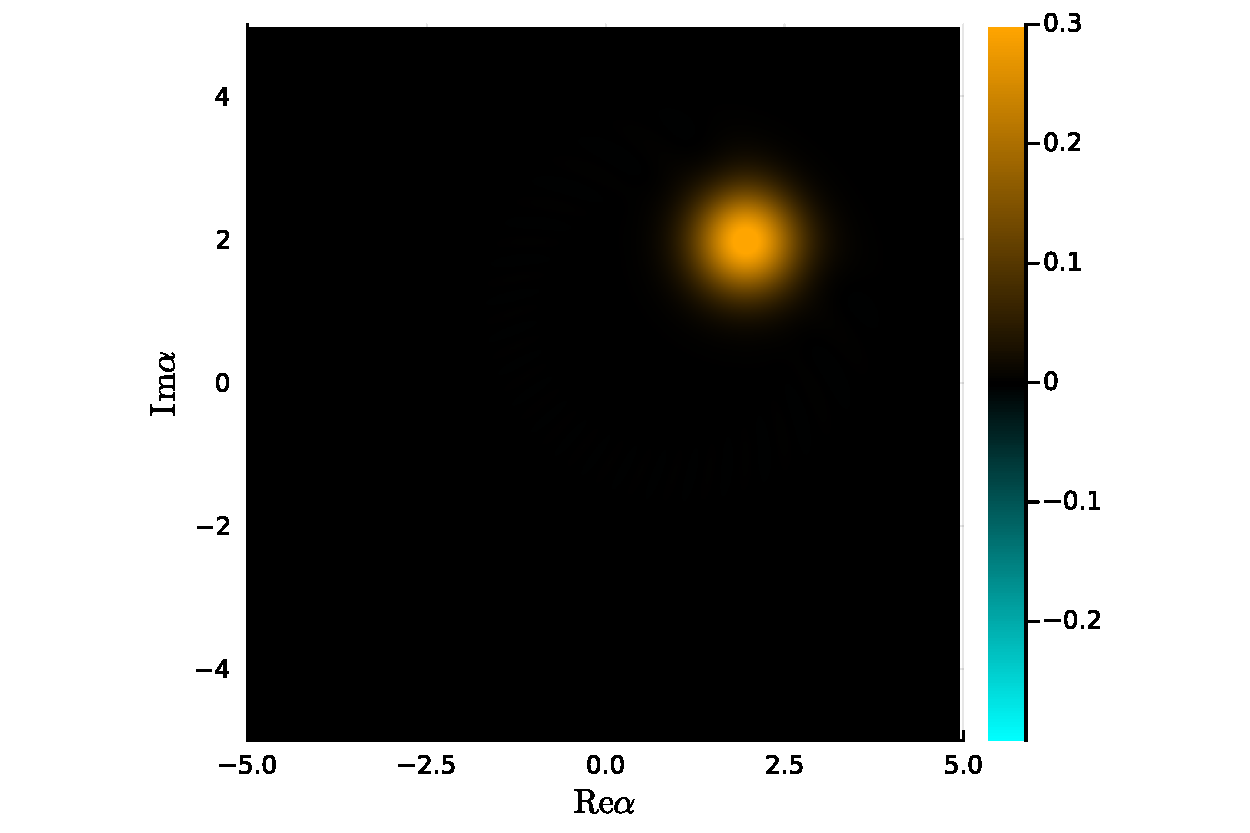
\includegraphics[width=\textwidth]{heatmaps/coherent-state2.pdf}
        \subcaption{}
    \end{subfigure}
    \begin{subfigure}{0.45\textwidth}
        \centering
        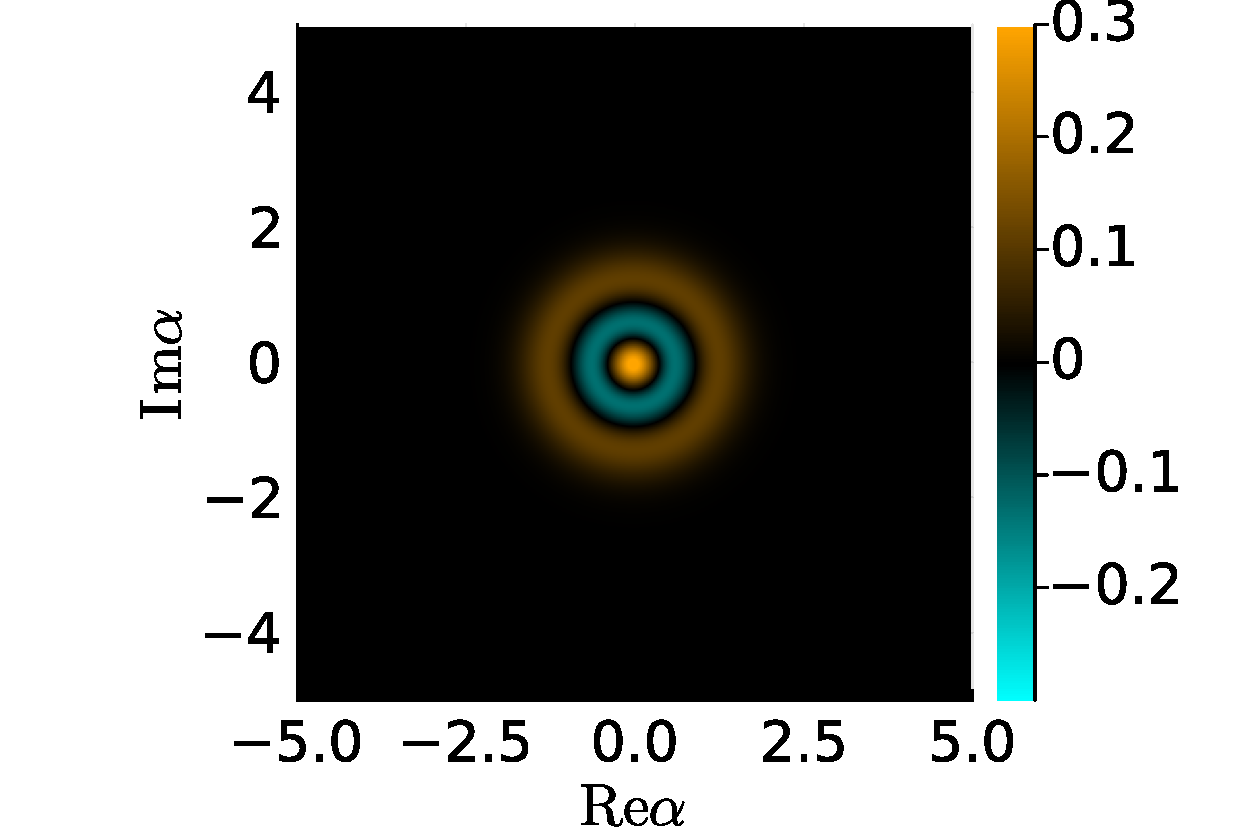
\includegraphics[width=\textwidth]{heatmaps/fock-state.pdf}
        \subcaption{}
    \end{subfigure}
    \begin{subfigure}{0.45\textwidth}
        \centering
        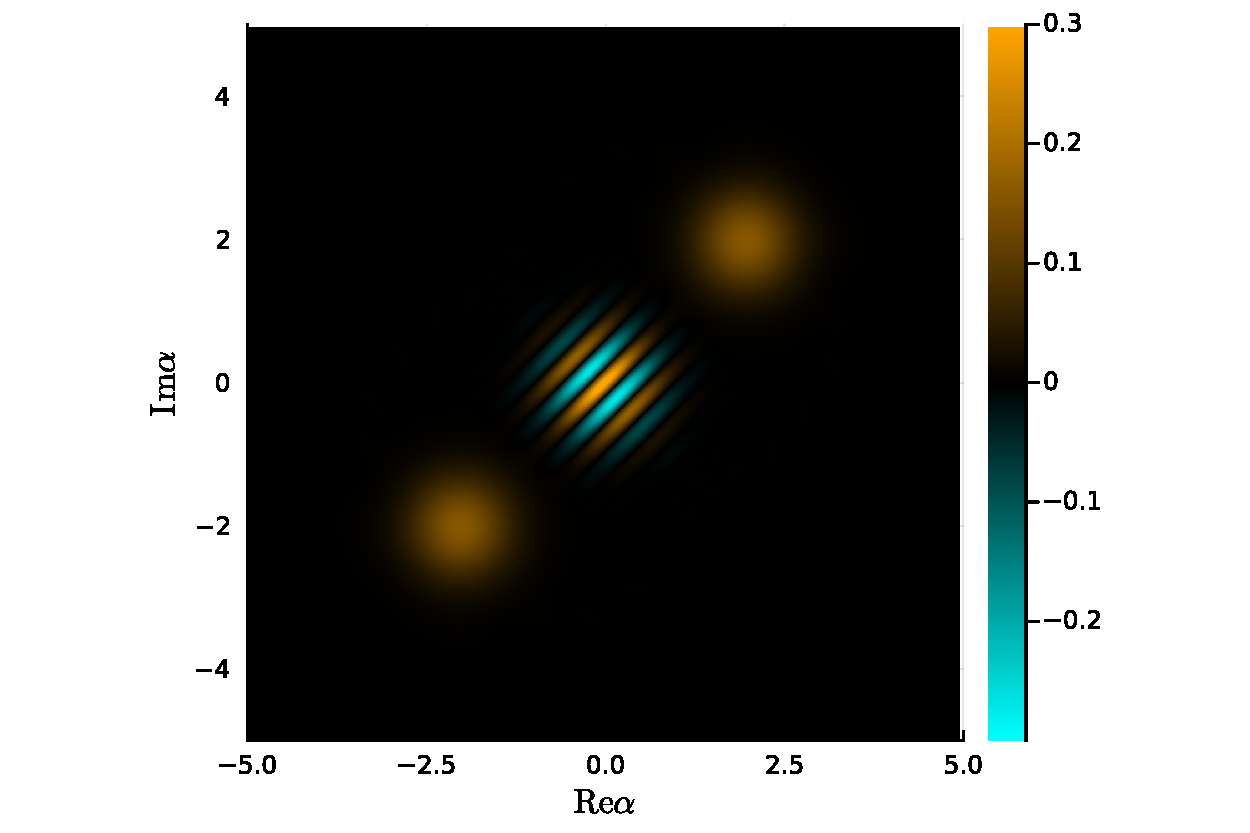
\includegraphics[width=\textwidth]{heatmaps/coherent-state-composition.pdf}
        \subcaption{} 
    \end{subfigure}
    \begin{subfigure}{0.45\textwidth}
        \centering
        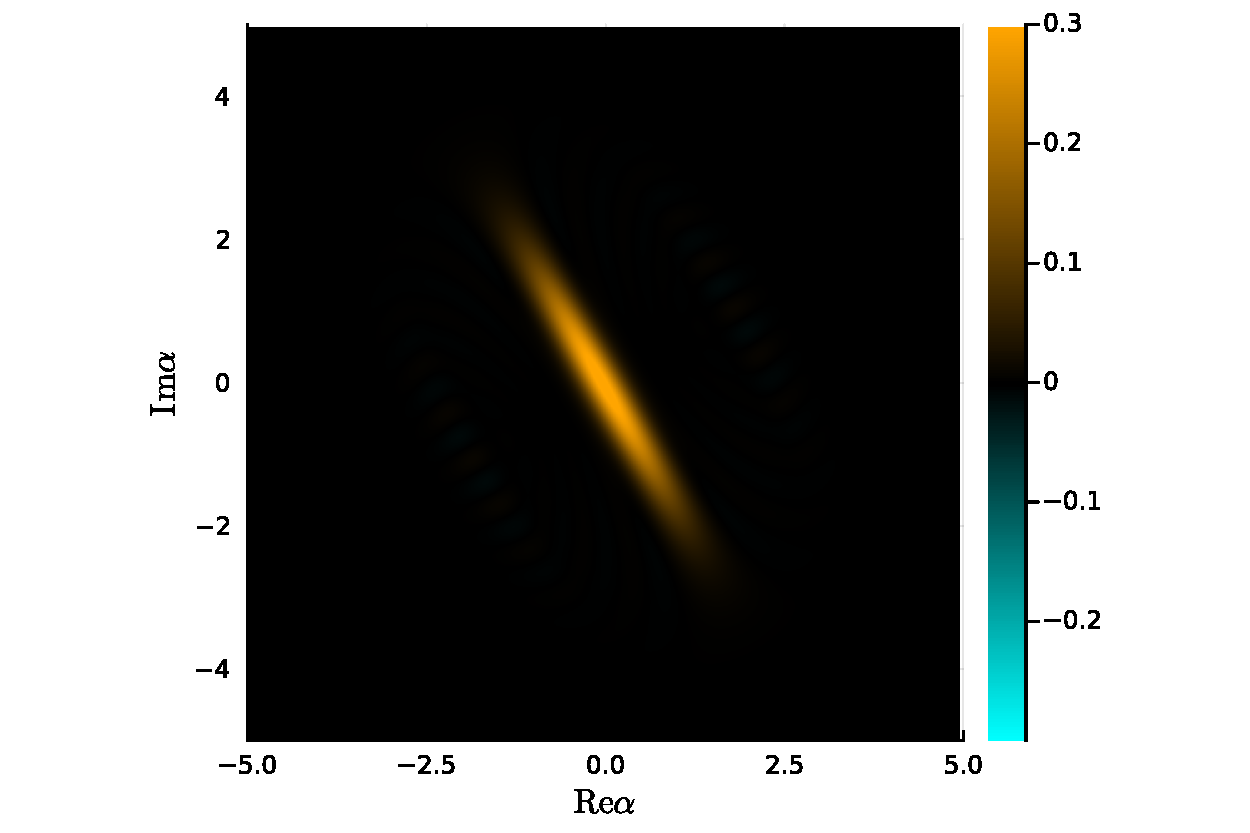
\includegraphics[width=\textwidth]{heatmaps/squeezed-state.pdf}
        \subcaption{}
    \end{subfigure}
    \begin{subfigure}{0.45\textwidth}
        \begin{tikzpicture}[x=0.75pt,y=0.75pt,yscale=-0.8,xscale=0.8]
    %uncomment if require: \path (0,300); %set diagram left start at 0, and has height of 300
    
    %Straight Lines [id:da13141330406552099] 
    \draw    (109,158) -- (352.5,158) ;
    \draw [shift={(354.5,158)}, rotate = 180] [fill={rgb, 255:red, 0; green, 0; blue, 0 }  ][line width=0.08]  [draw opacity=0] (12,-3) -- (0,0) -- (12,3) -- cycle    ;
    %Straight Lines [id:da7544554659071903] 
    \draw    (231.75,247.14) -- (231.75,70.86) ;
    \draw [shift={(231.75,68.86)}, rotate = 90] [fill={rgb, 255:red, 0; green, 0; blue, 0 }  ][line width=0.08]  [draw opacity=0] (12,-3) -- (0,0) -- (12,3) -- cycle    ;
    %Shape: Ellipse [id:dp26846059007812917] 
    \draw  [draw opacity=0][fill={rgb, 255:red, 80; green, 227; blue, 194 }  ,fill opacity=0.5 ] (211.75,109.73) .. controls (221.95,105.5) and (239.18,123.68) .. (250.23,150.34) .. controls (261.27,177) and (261.96,202.04) .. (251.75,206.27) .. controls (241.55,210.5) and (224.32,192.32) .. (213.27,165.66) .. controls (202.23,139) and (201.54,113.96) .. (211.75,109.73) -- cycle ;
    %Straight Lines [id:da6012949089045287] 
    \draw  [dash pattern={on 0.84pt off 2.51pt}]  (228.97,98.99) -- (272.38,203.23) ;
    %Straight Lines [id:da06631462084820017] 
    \draw  [dash pattern={on 0.84pt off 2.51pt}]  (191.13,113.98) -- (237.53,224.68) ;
    %Straight Lines [id:da4862352418973601] 
    \draw    (237.16,220.83) -- (270.59,204.12) ;
    \draw [shift={(272.38,203.23)}, rotate = 153.43] [fill={rgb, 255:red, 0; green, 0; blue, 0 }  ][line width=0.08]  [draw opacity=0] (12,-3) -- (0,0) -- (12,3) -- cycle    ;
    \draw [shift={(235.38,221.73)}, rotate = 333.43] [fill={rgb, 255:red, 0; green, 0; blue, 0 }  ][line width=0.08]  [draw opacity=0] (12,-3) -- (0,0) -- (12,3) -- cycle    ;
    %Straight Lines [id:da13038407369983673] 
    \draw  [dash pattern={on 0.84pt off 2.51pt}]  (165.94,188.16) -- (297.56,127.84) ;
    %Curve Lines [id:da1317810618305646] 
    \draw    (283.88,157.73) .. controls (284.11,152.27) and (283.45,149.96) .. (278.66,139.03) ;
    \draw [shift={(277.88,137.23)}, rotate = 66.25] [fill={rgb, 255:red, 0; green, 0; blue, 0 }  ][line width=0.08]  [draw opacity=0] (12,-3) -- (0,0) -- (12,3) -- cycle    ;
    %Straight Lines [id:da7382183063594989] 
    \draw  [dash pattern={on 0.84pt off 2.51pt}]  (184.63,122.65) -- (227.88,101.31) ;
    %Straight Lines [id:da7491733898506188] 
    \draw  [dash pattern={on 0.84pt off 2.51pt}]  (224.63,220.15) -- (269.1,197.85) ;
    %Straight Lines [id:da1580018626163433] 
    \draw    (187.63,122.75) -- (226.12,216.55) ;
    \draw [shift={(226.88,218.4)}, rotate = 247.69] [fill={rgb, 255:red, 0; green, 0; blue, 0 }  ][line width=0.08]  [draw opacity=0] (12,-3) -- (0,0) -- (12,3) -- cycle    ;
    \draw [shift={(186.88,120.9)}, rotate = 67.69] [fill={rgb, 255:red, 0; green, 0; blue, 0 }  ][line width=0.08]  [draw opacity=0] (12,-3) -- (0,0) -- (12,3) -- cycle    ;
    
    % Text Node
    \draw (253.88,225.21) node [anchor=north west][inner sep=0.75pt]    {$\frac{1}{2}\mathrm{e}^{-r}$};
    % Text Node
    \draw (297.88,143.93) node [anchor=west] [inner sep=0.75pt]    {$\theta /2$};
    % Text Node
    \draw (356.5,158) node [anchor=west] [inner sep=0.75pt]    {$\Re \alpha $};
    % Text Node
    \draw (231.75,65.46) node [anchor=south] [inner sep=0.75pt]    {$\Im \alpha $};
    % Text Node
    \draw (174.88,185.13) node [anchor=north west][inner sep=0.75pt]    {$\frac{1}{2}\mathrm{e}^{r}$};
    
    
    \end{tikzpicture}
    
        \subcaption{}
    \end{subfigure}
    \caption{Wigner functions in quantum optics. 
    Figures are plotted using \texttt{QuantumOptics.jl} \cite{kramer2018quantumoptics}.
    (a) The Wigner function of the vacuum. Note that this is not a $\delta$-function located at $\alpha = 0$.
    (b) The Wigner function of $\ket{\alpha = 2 + 2\ii}$.
    (c) The Wigner function of a single-photon state. Negative values occur.
    (d) The Wigner function of $(\ket{\alpha = 2 + 2 \ii} + \ket{\alpha = - 2 - 2 \ii}) / \sqrt{2}$.
    (e) The Wigner function of $S(\ee^{\ii \frac{\pi}{3}}) \ket{0}$.
    (f) Schematic illustration of the Wigner function of a squeezed vacuum state
    $S(r\ee^{\ii \theta}) \ket{0}$.
    The uncertainty relation \eqref{eq:re-im-fluctuation} is observed.
    The diagram is adapted from Fig. 2.8 in \cite{scully1999quantum}.
    }
    \label{fig:wigner-example}
\end{figure}

In linear quantum optics, we have \cite{steck2007quantum} 
\begin{equation}
    H = \int \dd[3]{\vb*{r}} \left( \frac{1}{2} \epsilon \vb*{E}^2 + \frac{1}{2 \mu} \vb*{B}^2 \right)
    = \sum_{k} \omega_k \left( a^\dagger_k a_k + \frac{1}{2} \right),
\end{equation}
where $k$ is the label of the optical normal mode $\vb*{f}_k$ and 
\begin{equation}
    \boldsymbol{E}=\sum_k \mathcal{E}_k \boldsymbol{f}_k a_k \mathrm{e}^{-\mathrm{i} \omega_k t}+\text {h.c.} , \quad 
    \mathcal{E}_k = \sqrt{\frac{\hbar \omega_k}{2 \epsilon_0 V}} , \quad \frac{1}{V} \int \mathrm{d}^3 \boldsymbol{r} \boldsymbol{f}_{k'}^* \cdot \frac{\boldsymbol{\epsilon}}{\epsilon_0} \cdot \boldsymbol{f}_k =\delta_{k k'} .
\end{equation}
The label $k$ is the momentum and polarization in a large box, 
and in an spherical optical cavity, it labels spherical harmonics.
We have the standard bosonic commutation relations 
\begin{equation}
    \comm*{a_k}{a_{k'}} = 0, \quad \comm*{a_k}{a^\dagger_{k'}} = \delta_{k k'}.
\end{equation}

To visualize a quantum state and the quantum noise in it,
so-called quasi-probability distribution functions may be utilized.
For one mode, if $a$ and $a^\dagger$ in an arbitrary operator $O$ is ordered according to a certain convention
($a$ before $a^\dagger$, or $a^\dagger$ before $a$, 
or whenever multiplication appears, it is in the form of $(a^\dagger a + a a^\dagger) / 2$), 
we have 
\begin{equation}
    \expval*{O(a, a^\dagger)} = \int \dd[2]{\alpha} f(\alpha, \alpha^*) O(\alpha, \alpha^*),
\end{equation}
where $O(\alpha, \alpha^*)$ is the 
polynomial form of $O$ in terms of $a, a^\dagger$ with the correct ordering
applied to dummy variables $\alpha$ and $\alpha^*$.
Here $\alpha$ can be roughly conceived as the ``value'' of $a$.
We say $f(\alpha, \alpha^*)$ is a quasi-probability distribution function.
Note that this definition even extends to the case 
when we are in a mixed state instead of a pure state, 
i.e. it is a unified treatment of both quantum noise and thermal noise.

To plot the function as a 2D heatmap,
it is often more convenient to change the coordinates into $\Re \alpha$ and $\Im \alpha$.
Note that we have 
\begin{equation}
    \comm*{\Re a}{\Im a} = \frac{1}{4 \ii} \comm*{a + a^\dagger}{a - a^\dagger}
    = \frac{\ii}{2},
\end{equation}
and according to the uncertainty principle, we have 
\begin{equation}
    \Delta (\Re a) \cdot \Delta (\Im a) \geq \frac{1}{4}.
    \label{eq:re-im-fluctuation}
\end{equation}
Another frequent convention is to define 
\begin{equation}
    a = \frac{1}{\sqrt{2}} (X + \ii P), \quad 
    a^\dagger = \frac{1}{\sqrt{2}} (X - \ii P),
    \label{eq:xy-to-a}
\end{equation}
and we find $\comm*{X}{P} = \ii$.
Here the $\sqrt{2}$ factor is simply there to normalize the commutation relation.

The most famous quasi-probability distribution is probably the \concept{Wigner function},
and it is the quasi-probability distribution used in this report.
The Wigner function of a density matrix $\rho$ (which is $\dyad{\psi}$ for a pure state) 
is defined as \cite{scully1999quantum}
\begin{equation}
    W(x, p)=\frac{1}{\pi \hbar} \int_{-\infty}^{\infty}\langle x-y|{\rho}| x+y\rangle e^{-2 \ii p y / \hbar} \dd y,
\end{equation}
and we can use \eqref{eq:xy-to-a} to define $W(\alpha, \alpha^*)$ and hence $W(\Re \alpha, \Im \alpha)$.

Some examples of pure state Wigner functions are given in \prettyref{fig:wigner-example}.
\prettyref{fig:wigner-example}(a) is the Wigner function of the vacuum state:
there is no photon, 
and the distribution of probability is focused on $\alpha = 0$.
Note that it is not a $\delta$-function,
and is somehow ``blurred'':
this is a visualization of \eqref{eq:re-im-fluctuation}.
Not all two-variable functions can be a Wigner function:
they cannot have too strong ``spatial resolution''.
The vacuum state is a specific case of the family of \concept{coherent states}.
A coherent state labeled by the complex parameter $\alpha$ is defined as 
\begin{equation}
    \ket{\alpha} = D(\alpha) \ket{0} = \ee^{\alpha a - \alpha^* a^\dagger} \ket{0},
    \quad a \ket{\alpha} = \alpha \ket{\alpha}.
\end{equation}
In the classical limit, 
the electric field of a light field in $\ket{\alpha}$
is $\vb*{E} = \alpha \vb*{f} \ee^{- \ii \omega t} + \text{c.c.}$,
where $\vb*{f}$ is the mode function.
\prettyref{fig:wigner-example}(d) is an example of a coherent state with $\alpha \neq 0$.
\prettyref{fig:wigner-example}(c) and (d) 
are Wigner functions of a Fock state (i.e. an eigenstate of $n = a^\dagger a$)
and a superposition state of two coherent states.
We have $\expval*{\vb*{E}} = 0$ for a Fock state,
because $\expval*{a}{n} = 0$,
but $\expval*{\vb*{E}^2} \neq 0$.
\prettyref{fig:wigner-example}(d) is a prototypical ``cat'' state.
Therefore both of them are far from classical states,
and correspondingly the Wigner functions of them have negative values,
which is impossible for a classical probability distribution.
\prettyref{fig:wigner-example}(e) is a ``squeezed vacuum''.
To squeeze a state with the complex parameter $\xi$ means to apply 
\begin{equation}
    S(\xi) = \ee^{\frac{1}{2} (\xi^* a^2 - \xi (a^\dagger)^2)}
\end{equation}
to that state.
The schematic Wigner function of a squeezed vacuum state 
with parameter $\xi = r \ee^{\ii \theta}$
is illustrated in \prettyref{fig:wigner-example}(f).
It can be seen that with $S(\xi) \ket{0}$, 
we have \cite{scully1999quantum}
\begin{equation}
    \Delta \left( \cos \frac{\theta}{2} \Re a  + \sin \frac{\theta}{2} \Im a \right)  = \frac{1}{2} \ee^{-r},
    \label{eq:min-op-squeeze}
\end{equation} 
while 
\begin{equation}
    \Delta \left( \sin \frac{\theta}{2} \Re a - \cos \frac{\theta}{2} \Im a \right) = \frac{1}{2} \ee^{r}.
\end{equation}


\section{Quantum noise in the Mach-Zehnder interferometer}\label{sec:interferometer}

\begin{figure}
    \centering
    \begin{tikzpicture}[x=0.75pt,y=0.75pt,yscale=-1,xscale=1]
    %uncomment if require: \path (0,300); %set diagram left start at 0, and has height of 300
    
    %Shape: Square [id:dp5396904315538396] 
    \draw   (153,108) -- (127,108) -- (127,134) -- (153,134) -- cycle ;
    %Straight Lines [id:da8471914401201053] 
    \draw    (153,134) -- (127,108) ;
    
    %Straight Lines [id:da7935401918038376] 
    \draw    (60,121) -- (140,121) ;
    \draw [shift={(100,121)}, rotate = 180] [fill={rgb, 255:red, 0; green, 0; blue, 0 }  ][line width=0.08]  [draw opacity=0] (12,-3) -- (0,0) -- (12,3) -- cycle    ;
    %Straight Lines [id:da12011802802769855] 
    \draw    (140,121) -- (140,188.67) ;
    \draw [shift={(140,154.83)}, rotate = 270] [fill={rgb, 255:red, 0; green, 0; blue, 0 }  ][line width=0.08]  [draw opacity=0] (12,-3) -- (0,0) -- (12,3) -- cycle    ;
    %Straight Lines [id:da45241792789009994] 
    \draw    (140,66.62) -- (140,121) ;
    \draw [shift={(140,93.81)}, rotate = 270] [fill={rgb, 255:red, 0; green, 0; blue, 0 }  ][line width=0.08]  [draw opacity=0] (12,-3) -- (0,0) -- (12,3) -- cycle    ;
    %Straight Lines [id:da5153136174085808] 
    \draw    (140,121) -- (220,121) ;
    \draw [shift={(180,121)}, rotate = 180] [fill={rgb, 255:red, 0; green, 0; blue, 0 }  ][line width=0.08]  [draw opacity=0] (12,-3) -- (0,0) -- (12,3) -- cycle    ;
    %Shape: Square [id:dp7233820176028007] 
    \draw   (384,177) -- (358,177) -- (358,203) -- (384,203) -- cycle ;
    %Straight Lines [id:da4232871242423555] 
    \draw    (384,203) -- (358,177) ;
    
    %Shape: Rectangle [id:dp8767012605022662] 
    \draw   (219.71,105.12) -- (289.71,105.12) -- (289.71,136) -- (219.71,136) -- cycle ;
    %Straight Lines [id:da4420821653329212] 
    \draw    (140,189) -- (371,189) ;
    \draw [shift={(255.5,189)}, rotate = 180] [fill={rgb, 255:red, 0; green, 0; blue, 0 }  ][line width=0.08]  [draw opacity=0] (12,-3) -- (0,0) -- (12,3) -- cycle    ;
    %Straight Lines [id:da5818295505336346] 
    \draw    (290,121) -- (370,121) ;
    \draw [shift={(330,121)}, rotate = 180] [fill={rgb, 255:red, 0; green, 0; blue, 0 }  ][line width=0.08]  [draw opacity=0] (12,-3) -- (0,0) -- (12,3) -- cycle    ;
    %Straight Lines [id:da06983065057757765] 
    \draw    (353.98,104.98) -- (386.02,137.02) ;
    %Straight Lines [id:da7059684030986733] 
    \draw    (123.98,172.65) -- (156.02,204.69) ;
    %Straight Lines [id:da18624562535781375] 
    \draw    (371,122.33) -- (371,190) ;
    \draw [shift={(371,156.17)}, rotate = 270] [fill={rgb, 255:red, 0; green, 0; blue, 0 }  ][line width=0.08]  [draw opacity=0] (12,-3) -- (0,0) -- (12,3) -- cycle    ;
    %Straight Lines [id:da06098229649677367] 
    \draw    (371,189) -- (451,189) ;
    \draw [shift={(411,189)}, rotate = 180] [fill={rgb, 255:red, 0; green, 0; blue, 0 }  ][line width=0.08]  [draw opacity=0] (12,-3) -- (0,0) -- (12,3) -- cycle    ;
    %Straight Lines [id:da7157358634488349] 
    \draw    (371,190) -- (371,253.73) ;
    \draw [shift={(371,221.86)}, rotate = 270] [fill={rgb, 255:red, 0; green, 0; blue, 0 }  ][line width=0.08]  [draw opacity=0] (12,-3) -- (0,0) -- (12,3) -- cycle    ;
    
    % Text Node
    \draw (254.71,120.56) node    {$\mathrm{e}^{\mathrm{i} 2\varphi }$};
    % Text Node
    \draw (108,86.4) node [anchor=north west][inner sep=0.75pt]    {$S_{1}$};
    % Text Node
    \draw (386,206.4) node [anchor=north west][inner sep=0.75pt]    {$S_{2}$};
    % Text Node
    \draw (42,109.4) node [anchor=north west][inner sep=0.75pt]    {$a_{1}^{\dagger }$};
    % Text Node
    \draw (133,43.4) node [anchor=north west][inner sep=0.75pt]    {$a_{2}^{\dagger }$};
    % Text Node
    \draw (458,176.4) node [anchor=north west][inner sep=0.75pt]    {$b_{2}^{\dagger }$};
    % Text Node
    \draw (366,262.4) node [anchor=north west][inner sep=0.75pt]    {$b_{1}^{\dagger }$};
    
    
    \end{tikzpicture}
    
    \caption{The schematic structure of the Mach-Zehnder interferometer}
    \label{fig:mz-inter}
\end{figure}

To have a concrete example of quantum noise, 
let us move to the \concept{Mach-Zehnder interferometer} \cite{caves_quantum-mechanical_1981},
illustrated in \prettyref{fig:mz-inter}.
The interferometer contains two beam splitters, 
two ideal mirrors, 
and one sample that introduces a $2\varphi$ phase shift to the light beam going through it.
The two beams created by the first beam splitter gain a phase difference caused by the sample,
and are then remixed together by the second beam splitter,
so there is interference,
and $\varphi$ can be found by comparing the output signal with the injected laser beam.

We are going to work in the Heisenberg picture,
because the whole system is linear 
and time evolution can be easily described by a linear transformation on the operators. 
Since this section is just to exemplify the overall idea of quantum noise,
for the sake of simplicity we assume the time evolution operator of the beam splitter is 
\begin{equation}
    S_{\text{beam splitter}} = \frac{1}{\sqrt{2}} \pmqty{ 1 & 1 \\ -1 & 1 } .
\end{equation}
The time evolution operator of the whole system is therefore
\begin{equation}
    \begin{aligned}
        S_\text{total}(\varphi) &= \frac{1}{\sqrt{2}} \pmqty{ 1 & -1 \\ 1 & 1 } \cdot \pmqty{\dmat{\ee^{\ii \varphi}, \ee^{- \ii \varphi}}} \cdot \frac{1}{\sqrt{2}} \pmqty{ 1 & 1 \\ -1 & 1 } \\
        &= \pmqty{ \cos \varphi & \ii \sin \varphi \\ - \ii \sin \varphi & - \cos \varphi },
    \end{aligned}
    \label{eq:total-matrix}
\end{equation} 
and therefore%
\footnote{
    Note that the EOM of the annihilation operators in the Heisenberg picture 
    has the same form with the EOM of the wave function in the Schr\={o}dinger picture.
} 
\begin{equation}
    \pmqty{b_1 \\ b_2} = \pmqty{ \cos \varphi & \ii \sin \varphi \\ - \ii \sin \varphi & - \cos \varphi } \pmqty{a_1 \\ a_2}, \quad 
    \pmqty{b_1^\dagger \\ b_2^\dagger} = \pmqty{ \cos \varphi & - \ii \sin \varphi \\ \ii \sin \varphi & - \cos \varphi } \pmqty{a_1^\dagger \\ a_2^\dagger},
    \label{eq:b-def-by-a}
\end{equation}
from which we find 
\begin{equation}
    \pmqty{a_1^\dagger \\ a_2^\dagger} = \pmqty{ \cos \varphi & - \ii \sin \varphi \\ \ii \sin \varphi & - \cos \varphi } \pmqty{b_1^\dagger \\ b_2^\dagger}.
\end{equation}
In actual experiment settings,
usually a beam of laser is injected into input port 1,
so the state at input port 1 is a coherent state.
Then, the wave function is 
\begin{equation}
    \begin{aligned}
        \ket{\psi} &= \underbrace{\ee^{\alpha a_1 - \alpha^* a_1^\dagger}}_{D_{a_1}(\alpha)} \ket{0} \\
        &= \ee^{\alpha (\cos \varphi b_1^\dagger - \ii \sin \varphi b_2^\dagger) -\alpha^{*} (\cos \varphi b_1 + \ii \sin \varphi b_2)}|0\rangle \\
        &= D_{b_1} (\alpha \cos \varphi) D_{b_2} (- \ii \alpha \sin \varphi) \ket{0} .
    \end{aligned}
    \label{eq:out-state}
\end{equation}
Note that the state in $a_2$ subspace remains vacuum;
it is a convention to call $a_2$ the \concept{dark port}.

The next step is measurement.
For simplicity we assume $\varphi \ll 1$,
and therefore the signal in the $b_2$ mode is $\sim \varphi$,
while the signal in the $b_1$ mode is $\sim \varphi^2$
(the signal in the $b_1$ mode should be defined as $\alpha - \alpha \cos \varphi$).
So we consider the expectation of $n_{b_2}$, which is
\begin{equation}
    \expval{n_{b_2}} = \abs{\alpha}^2 \sin^2 \varphi.
    \label{eq:output-exp}
\end{equation}
This output comes with a quantum uncertainty, which is given by 
\begin{equation}
    \begin{aligned}
        \Delta n_{b_2} &= \sqrt{ \expval*{n_{b_2}^2} - \expval*{n_{b_2}}^2 } \\
        &= \sqrt{ \expval*{ b_2^\dagger (b_2^\dagger b_2 + 1) b_2} - \expval*{n_{b_2}}^2 } \\
        &= \sqrt{ \abs{\alpha}^4 \sin^4 \varphi + \abs{\alpha}^2 \sin^2 \varphi - \abs{\alpha}^4 \sin^4 \varphi } \\
        &= \abs{\alpha} \sin \varphi.
    \end{aligned}
    \label{eq:stdvar-n2}
\end{equation}
Here we have used the property of coherent states as eigenstates of the annihilation operator.

So it can be seen that the relative uncertainty of the measurement is 
\begin{equation}
    \frac{\Delta n_{b_2}}{\expval{n_{b_2}}} 
    = \frac{\abs{\alpha} \sin \varphi}{\abs{\alpha}^2 \sin^2 \varphi} = \frac{1}{\sqrt{\expval*{n_{b_2}}}}.
    \label{eq:relvar-n2}
\end{equation}
It can be seen from \eqref{eq:stdvar-n2} that this standard error comes from 
the commutation relation $\comm*{b_2}{b_2^\dagger} = 1$,
which, eventually, comes from the fact that $\vb*{E}$ and $\vb*{A}$ in electromagnetism don't commute.
This is therefore a quantum noise.

Of course, \eqref{eq:relvar-n2} can be systematically reduced by increasing laser intensity,
so even if the quantum noise is always present, 
its influence can be progressively reduced.
But the detecting laser beam is another source of noise.
In the example of gravitational wave detection,
the mirrors used will be perturbed by the momenta of the photon jet arriving at them,
and since the number of photons has quantum fluctuation,
so is the motion of the mirrors,
and another noise is introduced to $\varphi$ \cite{caves1980quantum,abadie_gravitational_2011}.
(Note that this is true even when the mirrors are classical enough.) 
%TODO: back action described by Langevin equation
% We may say the mirrors observe the photons,
% and therefore the motion of them can be described by a Langevin equation
Classically,
we can successively weaken the laser beam 
and get an infinite sequence of measurements
with shrinking disturbance of the system,
the true value of the observable in question being the limit of this sequence.
But we know weakened laser beam means higher relative error 
introduced by the quantum noise.

Thus, astonishingly,
when quantum noise is present, 
even in principle, 
unboundedly improving the precision is not possible.
There is a non-zero minimal noise,
which is achieved when $\abs{\alpha}$ strikes a balance 
between the thermal fluctuation caused by large $\abs{\alpha}$
and quantum noise caused by small $\abs{\alpha}$ \cite{caves_quantum-mechanical_1981}.

%This actually makes sense,
%or otherwise we are faced with the problem 
%that an infinitely accurate continuous degree of freedom can store infinite bits of information.

\section{The quantum noise as the fluctuation of the dark port}\label{sec:dark-port-analysis}

One thing to keep in mind is \eqref{eq:relvar-n2} 
is about the quantum noise of the photon number, not others.
This quantity is not the only observable in $b_2$ mode,
but it is the only thing actually measured.
Thus it is possible that we reduce the quantum noise of $n_{b_2}$
and in exchange, get a larger quantum noise of other variables,
which we do not care.
This is called ``squeezing'' the quantum noise
-- the term will be visualized in the following discussion.
To do so, it is necessary to trace the origin of $\Delta{n_{b_2}}$ 
in terms of quantum noises of $a_1$ and $a_2$. 
For sake of simplicity,
here we keep the input state in the $a_1$ mode $\ket{\alpha}$,
without modifying anything,
and we also exclude all cross terms between $a_1$ and $a_2$ in the wave function, 
so we have 
\begin{equation}
    \ket{\psi} = D_{a_1}(\alpha) f(a_2, a_2^\dagger) \ket{0},
    \label{eq:coherent-plus-squeeze}
\end{equation}
and squeezing $\Delta{n_{b_2}}$ therefore reduces to squeezing the quantum noise of some operator in mode $a_2$.

From \eqref{eq:b-def-by-a}, we have 
\begin{equation}
    n_{b_2} = b_2^\dagger b_2 = 
    \sin^2 \varphi a_1^\dagger a_1 + \cos^2 \varphi a_2^\dagger a_2
    - \ii \sin \varphi \cos \varphi (a_1^\dagger a_2 - a_2^\dagger a_1).
    \label{eq:nb2-a}
\end{equation}
In the subspace determined by \eqref{eq:coherent-plus-squeeze},
all $a_1$ can be replaced by $\alpha$ in the above two equations,
but before that we should first complete normal ordering of $a_1$ and $a_1^\dagger$,
to include the non-trivial commutation relation of $a_1$
and thus the quantum fluctuation of the $a_1$ mode.
This however involves highly complicated calculation.

A huge simplification 
(and hence a neat explanation of the nature of the quantum noise in the interferometer) 
however can be made when $\varphi \ll 1$ and $\expval*{n_{a_2}} \ll \abs{\alpha}^2$.
The fluctuation of the first term in \eqref{eq:nb2-a} is $\sim \varphi^2 \abs{\alpha}$
(following \eqref{eq:stdvar-n2}),
whose order of $\varphi$ is higher than \eqref{eq:nb2-single-mode},
and therefore is suppressed,
although the $\expval*{\sin^2 \varphi a_1^\dagger a_1}$ term 
is the main contribution to $\expval*{n_{b_2}}$
and \eqref{eq:output-exp} is still correct,
because the expectations of the second and third terms are even smaller. 
The fluctuation of the second term in \eqref{eq:nb2-a} is also neglected,
because 
\begin{equation}
    \Delta (a_2^\dagger a_2)^2 = \expval*{ (a_2^\dagger a_2)^2 } - \expval*{ a_2^\dagger a_2 }^2 = 
    \expval*{a_2^\dagger a_2^\dagger a_2 a_2} + \expval*{a_2^\dagger a_2} - \expval*{ a_2^\dagger a_2 }^2 \simeq 0,
\end{equation}
compared with the absolute magnitude of 
$\Delta (a_1^\dagger a_1) = \abs{\alpha}$.
Under the above two conditions, approximately we have 
\begin{equation}
    \Delta n_{b_2} = \sin \varphi \cos \varphi \Delta (a_1^\dagger a_2 - a_2^\dagger a_1 ) .
\end{equation}
Since the input on the $a_1$ mode is much stronger than the input on the $a_2$ mode,
it is expected that the $a_1$ mode looks more classical and 
the quantum noise comes mainly from the $a_2$ mode,
which we can verify:
we have 
\[
    (a_1^\dagger a_2 - a_2^\dagger a_1)
    = a_1^\dagger a_2 a_1^\dagger a_2
    + a_2^\dagger a_1 a_2^\dagger a_1
    - \underbrace{a_2^\dagger a_1 a_1^\dagger a_2}_{a_2^\dagger a_2 a_1^\dagger a_1 + a_2^\dagger a_2}
    - \underbrace{a_1^\dagger a_2 a_2^\dagger a_1}_{a_1^\dagger a_1 a_2^\dagger a_2 + a_1^\dagger a_1},
\]
where the last two terms need normal ordering and therefore introduce quantum noise,
but the fourth term, which arises because of the commutation relation of $a_2$, 
is much larger than the third term,
because $\expval*{a_1^\dagger a_1} \gg \expval*{a_2^\dagger a_2}$,
and therefore we can treat $a_1$ classically.
Therefore we find the final expression of $\Delta n_{b_2}$: 
it is 
\begin{equation}
    \Delta n_{b_2} = \sin \varphi \cos \varphi \Delta (\alpha^* a_2 - \alpha a_2^\dagger)
    \approx \varphi \Delta (\alpha^* a_2 - \alpha a_2^\dagger).
    \label{eq:nb2-single-mode}
\end{equation}

We can do a sanity check:
if the $a_2$ state is vacuum,
then $\expval*{a_2} = \expval*{a_2^\dagger} = 0$, 
and again due to the non-trivial commutation relation, we have 
\begin{equation}
    \begin{aligned}
        \Delta n_{b_2} &\approx \varphi \Delta (\alpha^* a_2 - \alpha a_2^\dagger)
        = \varphi \sqrt{ \abs*{\expval*{ (\alpha^* a_2 - \alpha a_2^\dagger)^2 } 
        - \expval*{(\alpha^* a_2 - \alpha a_2^\dagger)}^2} } \\
        &= \varphi \sqrt{
            \abs{\alpha}^2 \expval*{a_2 a_2^\dagger}
        } 
        = \varphi \abs{\alpha} \sqrt{ 1 + \expval*{a^\dagger_2 a_2} } = \varphi \abs{\alpha},
    \end{aligned}
\end{equation}
which is the small-angle approximation of \eqref{eq:stdvar-n2}.

Note that \eqref{eq:nb2-single-mode} can also be written as  
\begin{equation}
    \begin{aligned}
        \Delta n_{b_2} &= \varphi \abs{\alpha} \Delta (\ee^{- \ii \phi} a_2 - \ee^{\ii \phi} a_2^\dagger)  \\
        &= \varphi \abs{\alpha} \Delta ( - 2 \ii \sin \phi \Re a_2 + 2 \ii \cos \phi \Im a_2 ) \\
        &= 2 \varphi \abs{\alpha} \Delta (- \sin \phi \Re a_2 + \cos \phi \Im a_2 ),
    \end{aligned}
    \label{eq:nb2-axis}
\end{equation}
where $\phi$ is the phase of $\alpha$.
The third line has a direct graphic meaning:
it has the form of \eqref{eq:min-op-squeeze}
and is proportion to the projection of the ``light spot'' in $W(\beta, \beta^*)$
on the axis (\prettyref{fig:can-be-squeezed})
\begin{equation}
    \cos \phi \Re \beta + \sin \phi \Im \beta = 0.
    \label{eq:measure-axis}
\end{equation}
Thus the quantum noise can be reduced by squeezing the variance on this axis,
while still keeping $\varphi \ll 1$ and 
$\abs{\alpha}^2 \gg \expval*{n_{a_2}}$.

\begin{figure}
    \centering
    \begin{subfigure}{0.48\textwidth}
        \centering
        \begin{tikzpicture}[x=0.75pt,y=0.75pt,yscale=-0.8,xscale=0.8]
    %uncomment if require: \path (0,300); %set diagram left start at 0, and has height of 300
    
    %Straight Lines [id:da04471469122433436] 
    \draw    (129,178) -- (372.5,178) ;
    \draw [shift={(374.5,178)}, rotate = 180] [fill={rgb, 255:red, 0; green, 0; blue, 0 }  ][line width=0.08]  [draw opacity=0] (12,-3) -- (0,0) -- (12,3) -- cycle    ;
    %Straight Lines [id:da015274839364082915] 
    \draw    (251.75,267.14) -- (251.75,90.86) ;
    \draw [shift={(251.75,88.86)}, rotate = 90] [fill={rgb, 255:red, 0; green, 0; blue, 0 }  ][line width=0.08]  [draw opacity=0] (12,-3) -- (0,0) -- (12,3) -- cycle    ;
    %Straight Lines [id:da40974022409973876] 
    \draw  [dash pattern={on 0.84pt off 2.51pt}]  (264.97,102.99) -- (308.38,207.23) ;
    %Straight Lines [id:da4130193128479054] 
    \draw  [dash pattern={on 0.84pt off 2.51pt}]  (179.13,126.98) -- (225.53,237.68) ;
    %Straight Lines [id:da39697617081453807] 
    \draw    (227.32,236.8) -- (304.86,198.89) ;
    \draw [shift={(306.65,198.01)}, rotate = 153.94] [fill={rgb, 255:red, 0; green, 0; blue, 0 }  ][line width=0.08]  [draw opacity=0] (12,-3) -- (0,0) -- (12,3) -- cycle    ;
    \draw [shift={(225.53,237.68)}, rotate = 333.94] [fill={rgb, 255:red, 0; green, 0; blue, 0 }  ][line width=0.08]  [draw opacity=0] (12,-3) -- (0,0) -- (12,3) -- cycle    ;
    %Straight Lines [id:da5963830448291811] 
    \draw  [dash pattern={on 0.84pt off 2.51pt}]  (185.94,208.16) -- (317.56,147.84) ;
    %Curve Lines [id:da3168543186358628] 
    \draw    (316.88,178.73) .. controls (317.65,185.74) and (313.55,189.69) .. (307.86,196.54) ;
    \draw [shift={(306.65,198.01)}, rotate = 309.02] [fill={rgb, 255:red, 0; green, 0; blue, 0 }  ][line width=0.08]  [draw opacity=0] (12,-3) -- (0,0) -- (12,3) -- cycle    ;
    %Shape: Polygon Curved [id:ds41898637181572873] 
    \draw  [draw opacity=0][fill={rgb, 255:red, 80; green, 227; blue, 194 }  ,fill opacity=0.2 ] (213,139) .. controls (233,129) and (208.5,92.06) .. (267.5,140.06) .. controls (326.5,188.06) and (264.13,181.98) .. (284.13,211.98) .. controls (304.13,241.98) and (233,229) .. (213,199) .. controls (193,169) and (193,149) .. (213,139) -- cycle ;
    
    % Text Node
    \draw (279.88,228.21) node [anchor=north west][inner sep=0.75pt]    {$\Delta n_{b_2}$};
    % Text Node
    \draw (320.38,187.18) node [anchor=west] [inner sep=0.75pt]    {$\phi $};
    % Text Node
    \draw (376.5,178) node [anchor=west] [inner sep=0.75pt]    {$\mathrm{Re} \alpha_2 $};
    % Text Node
    \draw (251.75,85.46) node [anchor=south] [inner sep=0.75pt]    {$\mathrm{Im} \alpha_2 $};
    
    
    \end{tikzpicture}
    
        \subcaption{}
    \end{subfigure}
    \begin{subfigure}{0.48\textwidth}
        \centering
        \begin{tikzpicture}[x=0.75pt,y=0.75pt,yscale=-0.8,xscale=0.8]
    %uncomment if require: \path (0,300); %set diagram left start at 0, and has height of 300
    
    %Straight Lines [id:da13141330406552099] 
    \draw    (109,158) -- (352.5,158) ;
    \draw [shift={(354.5,158)}, rotate = 180] [fill={rgb, 255:red, 0; green, 0; blue, 0 }  ][line width=0.08]  [draw opacity=0] (12,-3) -- (0,0) -- (12,3) -- cycle    ;
    %Straight Lines [id:da7544554659071903] 
    \draw    (231.75,247.14) -- (231.75,70.86) ;
    \draw [shift={(231.75,68.86)}, rotate = 90] [fill={rgb, 255:red, 0; green, 0; blue, 0 }  ][line width=0.08]  [draw opacity=0] (12,-3) -- (0,0) -- (12,3) -- cycle    ;
    %Shape: Ellipse [id:dp26846059007812917] 
    \draw  [draw opacity=0][fill={rgb, 255:red, 80; green, 227; blue, 194 }  ,fill opacity=0.5 ] (211.75,109.73) .. controls (221.95,105.5) and (239.18,123.68) .. (250.23,150.34) .. controls (261.27,177) and (261.96,202.04) .. (251.75,206.27) .. controls (241.55,210.5) and (224.32,192.32) .. (213.27,165.66) .. controls (202.23,139) and (201.54,113.96) .. (211.75,109.73) -- cycle ;
    %Straight Lines [id:da6012949089045287] 
    \draw  [dash pattern={on 0.84pt off 2.51pt}]  (228.97,98.99) -- (272.38,203.23) ;
    %Straight Lines [id:da06631462084820017] 
    \draw  [dash pattern={on 0.84pt off 2.51pt}]  (191.13,113.98) -- (237.53,224.68) ;
    %Straight Lines [id:da4862352418973601] 
    \draw    (237.16,220.83) -- (270.59,204.12) ;
    \draw [shift={(272.38,203.23)}, rotate = 153.43] [fill={rgb, 255:red, 0; green, 0; blue, 0 }  ][line width=0.08]  [draw opacity=0] (12,-3) -- (0,0) -- (12,3) -- cycle    ;
    \draw [shift={(235.38,221.73)}, rotate = 333.43] [fill={rgb, 255:red, 0; green, 0; blue, 0 }  ][line width=0.08]  [draw opacity=0] (12,-3) -- (0,0) -- (12,3) -- cycle    ;
    %Straight Lines [id:da13038407369983673] 
    \draw  [dash pattern={on 0.84pt off 2.51pt}]  (165.94,188.16) -- (297.56,127.84) ;
    %Curve Lines [id:da1317810618305646] 
    \draw    (283.88,157.73) .. controls (284.11,152.27) and (283.45,149.96) .. (278.66,139.03) ;
    \draw [shift={(277.88,137.23)}, rotate = 66.25] [fill={rgb, 255:red, 0; green, 0; blue, 0 }  ][line width=0.08]  [draw opacity=0] (12,-3) -- (0,0) -- (12,3) -- cycle    ;
    %Straight Lines [id:da7382183063594989] 
    \draw  [dash pattern={on 0.84pt off 2.51pt}]  (184.63,122.65) -- (227.88,101.31) ;
    %Straight Lines [id:da7491733898506188] 
    \draw  [dash pattern={on 0.84pt off 2.51pt}]  (224.63,220.15) -- (269.1,197.85) ;
    %Curve Lines [id:da3711544378836358] 
    \draw    (268.99,187.61) .. controls (278.37,178.63) and (286.37,174.2) .. (283.88,157.73) ;
    \draw [shift={(267.5,189.06)}, rotate = 315] [fill={rgb, 255:red, 0; green, 0; blue, 0 }  ][line width=0.08]  [draw opacity=0] (12,-3) -- (0,0) -- (12,3) -- cycle    ;
    
    % Text Node
    \draw (253.88,225.21) node [anchor=north west][inner sep=0.75pt]    {$\Delta n_{b_{2}} =\frac{1}{2}\mathrm{e}^{-r}$};
    % Text Node
    \draw (297.88,143.93) node [anchor=west] [inner sep=0.75pt]    {$\theta /2$};
    % Text Node
    \draw (356.5,158) node [anchor=west] [inner sep=0.75pt]    {$\mathrm{Re} \alpha_2 $};
    % Text Node
    \draw (231.75,65.46) node [anchor=south] [inner sep=0.75pt]    {$\mathrm{Im} \alpha_2 $};
    % Text Node
    \draw (293.88,180.93) node [anchor=west] [inner sep=0.75pt]    {$\varphi $};
    
    
    \end{tikzpicture}
    
        \subcaption{}
    \end{subfigure}
    \caption{Illustration of \eqref{eq:nb2-axis} in the Wigner phase space of $a_2$ mode. 
    (a) The variance of $n_{b_2}$ is the distance 
    between two $-\sin \phi \Re a_2 + \cos \phi \Im a_2 = C$ lines,
    or in other words the projection of the ``light spot'' on \eqref{eq:measure-axis}.
    (b) The Wigner function of a squeezed vacuum state injected into the dark port 
    to reduce quantum noise in the output.
    }
    \label{fig:can-be-squeezed}
\end{figure}

\section{Squeezing the quantum noise}\label{sec:squeezing}

If we inject a squeezed state with parameter $r \ee^{\ii \theta}$ 
into the dark port,
and let it has narrowest variation in the axis defined by \eqref{eq:measure-axis}, 
then we have 
\begin{equation}
    \frac{\theta}{2} - \phi = \frac{\pi}{2}.
    \label{eq:optimal-angle}
\end{equation}
This means if we increase $r$, 
the relative error seen in $n_{b_2}$ changes as 
(note that $\expval*{n_{b_2}}$ does not change,
and we have \eqref{eq:nb2-axis})
\begin{equation}
    \frac{\Delta n_{b_2}}{\expval*{n_{b_2}}} 
    \approx \frac{2 \abs{\alpha} \varphi \cdot \ee^{-r} /2 }{\abs{\alpha}^2 \varphi^2} 
    = \frac{1}{\abs{\alpha} \varphi} \ee^{-r}.
    \label{eq:approx-squeezing}
\end{equation}
Despite the exponent function factor,
injecting a squeezed state into the dark port however does not improve 
the precision of Mach-Zehnder interferometer endlessly:
when $\xi$ is very large,
the particle number expectation of the $a_2$ mode is no longer ignorable,
breaking one of the two conditions used to derive \eqref{eq:nb2-single-mode}.
This is illustrated in \prettyref{fig:squeezing},
where $\alpha = 2$, $\varphi = \pi / 10$,
and \eqref{eq:optimal-angle} is followed.
The initial difference between two plots arises because of the difference between $\varphi$ and $\sin \varphi$;
it can be seen that as $r$ exceeds 0.15,
the shapes of the two curves becomes different,
and in reality, increasing $r$ further actually increases the noise of $n_{b_2}$.
Full treatments of the output noise when the dark port receives a squeezed vacuum
can be found in \cite{walls_quantum_2008,pezze_mach-zehnder_2008} and references therein.

\begin{figure}
    \centering
    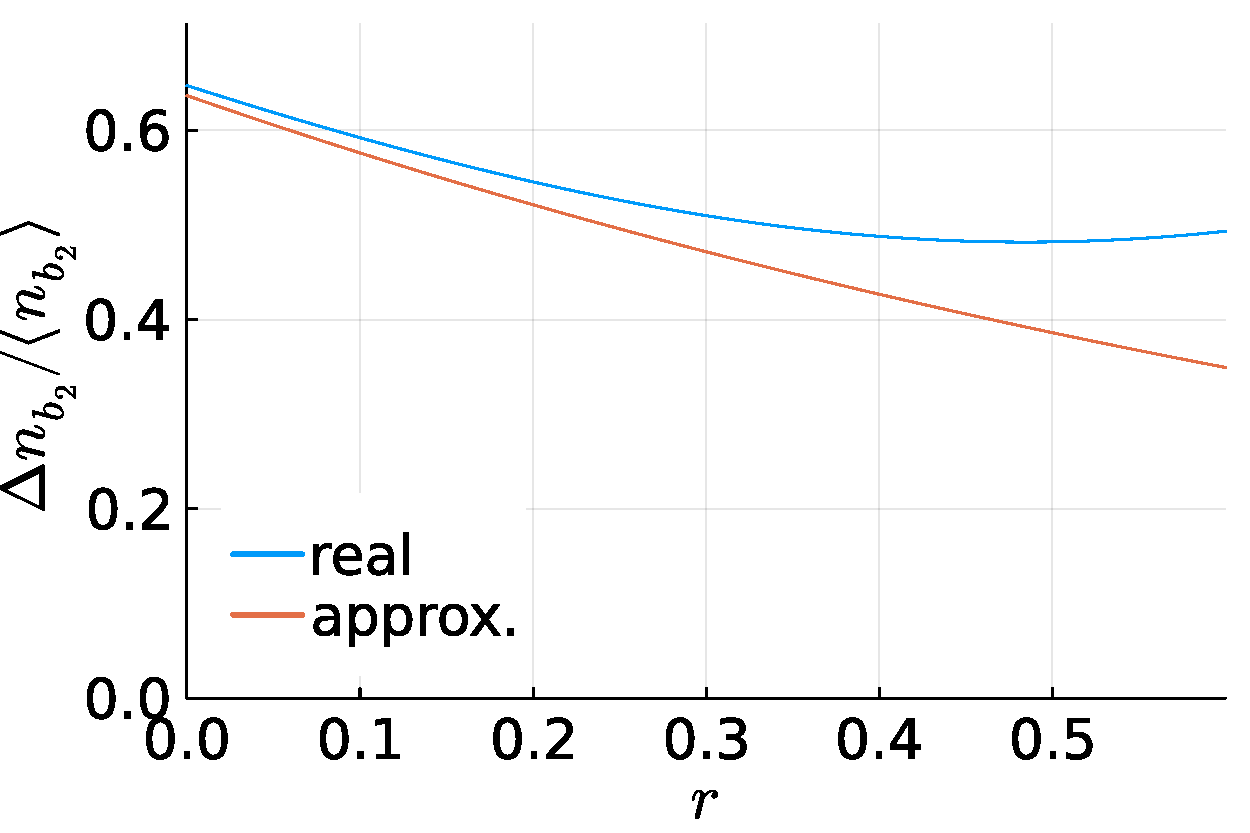
\includegraphics[width=0.49\textwidth]{plots/squeezing-error-measure-cutoff-50-phi-pi-10-alpha-5.pdf}
    \caption{Example of squeezed quantum noise: at $r = 0$ we have the standard quantum limit.
    Figure plotted using \texttt{QuantumOptics.jl} \cite{kramer2018quantumoptics}.
    In the ``real'' plot, 
    we calculate $\Delta n_{b_2}$ strictly by definition, 
    i.e. on the tensor product of the $a_1$ subspace and the $a_2$ subspace.
    The photon number cutoff for both spaces is 50,
    and $\alpha$ is set to 5.
    The ``approx.'' plot is drawn according to \prettyref{eq:approx-squeezing}.
    }
    \label{fig:squeezing}
\end{figure}

\section{Conclusion and discussion}

Unlike thermal noises arising from escape of information to the reservoir, 
quantum noise comes from the uncertain nature of physical quantities 
when we are dealing with a quantum state.
Despite its root in the basic laws of quantum mechanics,
quantum noises can be reduced by preparing appropriate initial states,
and a toy example is presented above in this report.

The protocol to squeeze quantum noises 
has already been demonstrated experimentally \cite{xiao_precision_1987},
and the breakdown of the squeezing scheme with strong squeezing outlined above 
can be avoided by extracting information from the fluctuation pattern of the output signal 
\cite{pezze_mach-zehnder_2008},
or with the so-called $N00N$ state \cite{giovannetti_advances_2011}. 
However, these protocols are bound by a $1 / N$ ($\simeq 1 / \abs{\alpha}^2$) quantum limit: 
the Heisenberg limit,
which roughly corresponds to the particle number-phase uncertainty principle:
what we measure is in essence a phase difference 
between two beams of light,
and then $\Delta \theta \sim 1 / \Delta N \sim 1 / N$,
though a more rigid proof is required \cite{giovannetti_quantum_2006}.
Despite often being depicted as the ultimate quantum limit,
by so-called nonlinear measurement, measurements beyond the Heisenberg limit are possible 
\cite{boixo2008quantum,napolitano_interaction-based_2011}.

A final remark on quantum noise squeezing is that 
the above disccusions are no longer illusory,
because the precisions of the most advanced gravitational wave detectors 
have already entered the region where quantum noises are important.
The squeezed state injection protocol has already been implemented on GEO 600 and LIGO 
\cite{abadie_gravitational_2011,aasi_enhanced_2013}
and resulted in expected reduction of noises.

\printbibliography

\end{document}